\subsection{Filtrage des étudiants redoublants et génération des contrats}

Dans le cadre de ce projet, nous avons développé un ensemble de scripts R visant à automatiser le processus de génération des contrats de redoublement à partir des données du jury. Ce processus se déroule en plusieurs étapes distinctes.

Après la création des fichiers \texttt{entete\_jury.xlsx} et \texttt{jury.xlsx}, il est nécessaire de générer automatiquement une liste de contrats de redoublement ainsi que des bilans, à partir de ces deux fichiers \texttt{xlsx}.

\subsection{Filtrage des étudiants redoublants}

La première étape consiste à écrire un script nommé \texttt{filtrerRedoublement.R}. Ce script permet d’identifier les étudiants susceptibles de redoubler, en se basant sur les données issues du fichier \texttt{entete\_jury.csv}. Il est important de noter que les simples moyennes présentes dans le fichier \texttt{jury.xlsx} ne suffisent pas à déterminer les cas de redoublement ; d’autres critères doivent être pris en compte, d’où l’utilisation de ce filtrage préalable.

\subsection{Récupération des noms et prénoms de tous les étudiants}

Ensuite, nous récupérons les noms et prénoms de tous les étudiants à partir du fichier \texttt{entete\_jury.xlsx}, grâce au script \texttt{RecupererNomPrenom.R}. Ces informations sont utilisées pour nommer individuellement les contrats générés dans la partie suivante, afin de bien distinguer chaque étudiant.

\subsection{Génération des contrats}

Une fois les étudiants redoublants identifiés, nous utilisons un script appelé \texttt{listeContratAlgo.R}. Celui-ci automatise l’appel à la fonction \texttt{generation()} définie dans le fichier \texttt{contrat\_notes.R}. Cette boucle permet de générer automatiquement un contrat de redoublement pour chaque étudiant concerné, en utilisant les données issues du fichier \texttt{jury.xlsx}. Chaque contrat est nommé à partir du nom et du prénom de l’étudiant, récupérés précédemment grâce au script \texttt{RecupererNomPrenom.R}.

\subsection{Production des bilans}

Enfin, une fois l’ensemble des contrats généré, nous produisons des bilans synthétiques à l’aide du script \texttt{bilan\_Algo.R}. Ces bilans sont générés pour :
\begin{itemize}
    \item le semestre 3 (S3),
    \item le semestre 4 (S4),
    \item et l’ensemble de l’année.
\end{itemize}

\begin{figure}[H]
  \centering
  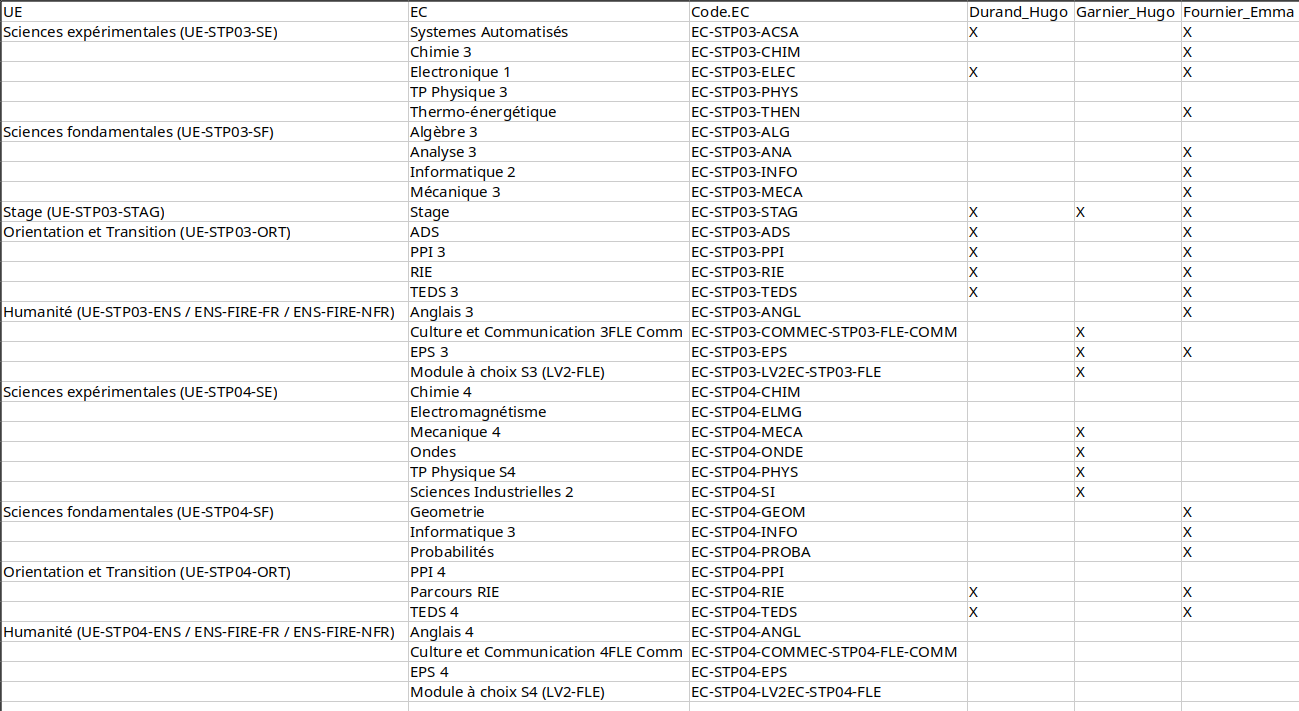
\includegraphics[width=\linewidth]{images/bilan.png}
  \caption{Extrait du bilan de l'ensemble de l'année}
  \label{generation_bilan}
\end{figure}

Ces bilans contiennent la liste des étudiants redoublants ainsi que les unités d’enseignement qu’ils devront repasser lors de la prochaine année universitaire. Ils constituent un outil précieux pour l’administration pédagogique dans le suivi des parcours étudiants.
